\documentclass[aspectratio=43]{beamer}
% \documentclass[aspectratio=169]{beamer}

% Title --------------------------------------------
\title[Lecture 1: Introduction to Research Design]{\Large Introduction to Research Design}
\author[]{Francisco Villamil}
\date[]{Research Design for Social Sciences\\MA Computational Social Science, UC3M\\Fall 2025}

\input{../beamer_preamble.tex}

\begin{document}
% ====================================================

% ----------------------------------------------------
\begin{frame}

  \titlepage

\end{frame}
% ----------------------------------------------------

% ----------------------------------------------------
\begin{frame}
\frametitle{Introduction}
\centering

\begin{itemize}
  \item<1-> What is this course about?
  \item<1-> Expectations?
  \item[]<2->
  \item<2-> \textbf{What is research? And why do we need to design it?}
\end{itemize}

\end{frame}
% ----------------------------------------------------

% ----------------------------------------------------
\begin{frame}
\frametitle{A real example}
\centering

\begin{itemize}[<+->]
  \item Racing team deciding whether to race or not in the last session
  \item Car engine has blown out in 7 out of 24 past races
  \begin{itemize}
    \item Should we risk an explosion and go bankrupt or race?
  \end{itemize}
  \item A mechanic has a last-minute gut feeling that it might have to do with temperature (forecast for race: very cold day)
  \item Someone says: ``show me the data of the past failures!''
\end{itemize}

\end{frame}
% ----------------------------------------------------

% ----------------------------------------------------
\imageframe{../img/challenger1}
% ----------------------------------------------------

% ----------------------------------------------------
\imageframe{../img/challenger2}
% ----------------------------------------------------

% ----------------------------------------------------
\imageframe{../img/challenger_wiki}
% ----------------------------------------------------

% ----------------------------------------------------
\begin{frame}
\frametitle{Challenger example}
\centering

\begin{itemize}
  \item \colorbox{yellow}{Explanatory} research
  \item What is the role of design here?
  \item<2-> Which observations to use
  \item<2-> What \textit{variation} we need to answer the question?
\end{itemize}

\end{frame}
% ----------------------------------------------------
  
% ----------------------------------------------------
\begin{frame}
\frametitle{Types of research}
\centering

\begin{itemize}
  \item \textit{Theoretical} and \colorbox{yellow}{\textit{empirical} research}
  \item<2-> \textit{Qualitative} and \colorbox{yellow}{\textit{quantitative} empirical research}
  \begin{itemize}
    \item<3-> Descriptive vs explanatory
  \end{itemize}
\end{itemize}

\end{frame}
% ----------------------------------------------------

% ----------------------------------------------------
\begin{frame}
\frametitle{Empirical Research}
\centering

\begin{itemize}
  \item Goal: answer a question using empirical evidence
  \begin{itemize}
    \item Usual problems: unanswerable questions, wrong data to question, concepts do not correspond to measurements...
  \end{itemize}
  \item<2-> How? exploiting \textbf{empirical variation}
  \item<2-> Research design is essentially knowing where to look at, how to measure it, how to analyze it, how to interpret it, etc --
  \item[]<2-> it's about \colorbox{yellow}{inference}
  \item<3-> Example:
    \begin{itemize}
      \item Hotel interested in increasing bookings
      \item Data used: online bookings and actual visits
    \end{itemize}
\end{itemize}

\end{frame}
% ----------------------------------------------------

% ----------------------------------------------------
\begin{frame}
\frametitle{Empirical research}
\centering

\begin{itemize}
  \item Usually includes many things we vaguely associate with ``data''
  \begin{itemize}
    \item Statistical analysis
    \item Experiments
    \item Simulations, cases without variation?
    \item etc
  \end{itemize}
  \item Idea is learning about \textbf{making claims}, or how can we learn from the observable world the right way
  \item Two things we should learn:
  \item[] how to answer questions \& and how to evaluate answers
\end{itemize}

\end{frame}
% ----------------------------------------------------

% ----------------------------------------------------
\begin{frame}
\frametitle{Empirical evidence and claims}
\centering

\includegraphics[width = 0.65\textwidth]{../img/nyt_museums}

\end{frame}
% ----------------------------------------------------

% ----------------------------------------------------
\begin{frame}
\frametitle{Empirical evidence and claims}
\centering

\begin{itemize}
  \item Let's reverse-engineer this:
  \begin{itemize}
    \item What did they probably do?
  \end{itemize}
  \item How would you answer the question better?
  \item<2-> Causal inference and experimental methods
  \begin{itemize}
    \item Observation vs manipulation
  \end{itemize}
  \item<3-> Gold standard?
\end{itemize}

\end{frame}
% ----------------------------------------------------
  
% ----------------------------------------------------
\imageframe{../img/psycho1}
% ----------------------------------------------------

% ----------------------------------------------------
\imageframe{../img/psycho2}
% ----------------------------------------------------

% ----------------------------------------------------
\imageframe{../img/psycho3}
% ----------------------------------------------------

% ----------------------------------------------------
\begin{frame}
\frametitle{Opinions about claims?}
\centering

\includegraphics[width = \textwidth]{../img/psycho4}

\end{frame}
% ----------------------------------------------------

% % ----------------------------------------------------
% \imageframe{../img/replicationcrisis1}
% % ----------------------------------------------------

% ----------------------------------------------------
\imageframe{../img/replicationcrisis2}
% ----------------------------------------------------

% ----------------------------------------------------
\imageframe{../img/marshmallow}
% ----------------------------------------------------

% ----------------------------------------------------
\imageframe{../img/marshmallow2}
% ----------------------------------------------------

% ----------------------------------------------------
\imageframe{../img/marshmallow3}
% ----------------------------------------------------

% ----------------------------------------------------
\begin{frame}
\frametitle{Other types of inference}
\centering

\begin{itemize}
  \item We are used to cases where we compare many observations with different values on key variables
  \item What if we don't have enough observations to answer a question?
  \item Any idea about examples?
\end{itemize}

\end{frame}
% ----------------------------------------------------
    

% ----------------------------------------------------
\imageframe{../img/derecho2022a}
% ----------------------------------------------------

% ----------------------------------------------------
\begin{frame}
\frametitle{Opinions? How do you think it's done?}
\centering

\includegraphics[width = \textwidth]{../img/derecho2022c}

\end{frame}
% ----------------------------------------------------

% ----------------------------------------------------
\imageframe{../img/derecho2022b}
% ----------------------------------------------------

% ----------------------------------------------------
\begin{frame}
\frametitle{Not only about data or empirical evidence}
\centering

\begin{itemize}
  \item The ``non-data'' part is also important:
  \item[] thinking about an answerable question, a coherent argument, and how to connect it to data
  \item[]
  \item Also problematic because we all probably think we already know how it's done, but e.g. many (most?) final theses fail on this
\end{itemize}

\end{frame}
% ----------------------------------------------------
  

% ----------------------------------------------------
\begin{frame}
\frametitle{Empirical Research process}
\centering

\resizebox{\linewidth}{!}{
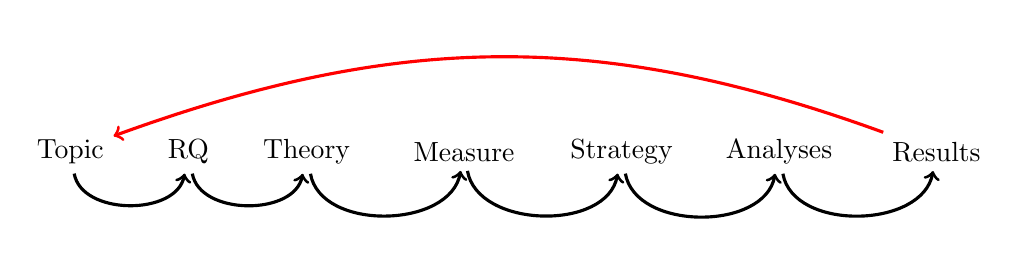
\begin{tikzpicture}
\node (topic) at (1,0) {Topic};
\node (rq) at (2.5,0) {RQ};
\node (theory) at (4,0) {Theory};
\node (measure) at (6,0) {Measure};
\node (strat) at (8,0) {Strategy};
\node (analyses) at (10,0) {Analyses};
\node (results) at (12,0) {Results};

\draw[->, line width=0.4mm] (topic) to[out=280, in=260] (rq) node[] {};
\draw[->, line width=0.4mm] (rq) to[out=280, in=260] (theory) node[] {};
\draw[->, line width=0.4mm] (theory) to[out=280, in=260] (measure) node[] {};
\draw[->, line width=0.4mm] (measure) to[out=280, in=260] (strat) node[] {};
\draw[->, line width=0.4mm] (strat) to[out=280, in=260] (analyses) node[] {};
\draw[->, line width=0.4mm] (analyses) to[out=280, in=260] (results) node[] {};
\draw[->, line width=0.4mm, red] (results) to[out=160, in=20] (topic) node[] {};

\end{tikzpicture}}

\end{frame}
% ----------------------------------------------------


% ----------------------------------------------------
\begin{frame}
\frametitle{Key ingredientes}
\centering

\begin{flushleft}
In every case, when we talk about \textit{quantitative empirical research}, we will usually work with \textbf{variation} across \textbf{observations} at a given \textbf{unit of analyses/observation}, from which we infer stuff
\end{flushleft}


\vspace{10pt}

\begin{itemize}[<+->]
  \item[1.] Observation
  \item[2.] Unit of analysis or unit of observation
  \item[3.] Variables
  \item[4.] Variation
\end{itemize}

\end{frame}
% ----------------------------------------------------

% ----------------------------------------------------
\begin{frame}<1>[label=variation]
\frametitle{A few questions on variation}
\centering

\begin{itemize}
  \item Why do we talk so much about \textit{variation}?
  \item<2-> Critique of having ``few observations''?
  \item<3-> Why do we use statistics at all?
  \item<4-> What about experiments?
  \item<5-> Where's the variation in attribution science?
\end{itemize}

\end{frame}
% ----------------------------------------------------

% ----------------------------------------------------
\imageframe{../img/halley_eclipse}
% ----------------------------------------------------

% ----------------------------------------------------
\againframe<2->{variation}
% ----------------------------------------------------

% ----------------------------------------------------
\begin{frame}
\frametitle{On the unit of analysis}
\centering

\begin{itemize}
  \item Why is this important?
  \item<2-> Able to quickly identify it?
\end{itemize}

\end{frame}
% ----------------------------------------------------
  

% ----------------------------------------------------
\begin{frame}
\frametitle{What's the unit of analyses in the data behind this graph?}
\centering

\includegraphics[width = 0.8\textwidth]{../img/ua1}

\end{frame}
% ----------------------------------------------------

% ----------------------------------------------------
\imageframe{../img/ua2}
% ----------------------------------------------------

% ----------------------------------------------------
\imageframe{../img/ua3}
% ----------------------------------------------------

% ----------------------------------------------------
\begin{frame}
\frametitle{On the unit of analysis}
\centering

\begin{itemize}
  \item Most empirical designs can be adapted to different units of analyses
  \item The unit you use is related to the question and theory
  \item Example: think again about the hotel that wants to increase bookings
  \begin{itemize}
    \item How many different units could you use and how are they related to different questions/theories?
  \end{itemize}
  \item<2-> Another example: children educational attainment and contextual factors (peers, school, family, etc)
\end{itemize}

\end{frame}
% ----------------------------------------------------

% ----------------------------------------------------
\begin{frame}
\frametitle{Reading}
\centering

\includegraphics[width = 0.8\textwidth]{../img/reading}

\end{frame}
% ----------------------------------------------------

% ----------------------------------------------------
\begin{frame}
\frametitle{Research process in detail (1)}
\centering

\begin{itemize}
  \item[$>$] From \textbf{topic} (or problem) to the \BGyellow{\textbf{research question}}
  \item[]
  \item<2-> Difference between motivation and question
  \item<3-> What are good \& bad research questions?
  \begin{itemize}
    \item Answerable
    \item Relevant: importance and connection theory/empirics (*)
  \end{itemize}
  \item[]<4->
  \item[]<4-> Examples, good and bad
  \begin{itemize}
    \item What is the best Netflix show?
    \item What can we do to help poor countries develop?
    \item What are the shopping patterns of the Spanish population?
    \item Do individuals from minorities support the use of violence?
  \end{itemize}
\end{itemize}

\end{frame}
% ----------------------------------------------------

% ----------------------------------------------------
\begin{frame}
\frametitle{Research process in detail (2)}
\centering

\begin{itemize}
  \item[$>$] From \textbf{RQ} to \BGyellow{\textbf{theory}}
  \item[]
  \item<2-> What is a theory? Importance
  \item<3-> Arguments and mechanisms
  \item<3-> Micro-level, macro-level, and both
  \item<4-> Good theories or arguments
  \begin{itemize}
    \item Testable
    \item Credible
  \end{itemize}
\end{itemize}

\end{frame}
% ----------------------------------------------------

% ----------------------------------------------------
\begin{frame}
\frametitle{Research process in detail (3)}
\centering

\begin{itemize}
  \item[$>$] From \textbf{theory} to \BGyellow{\textbf{measurement}}
  \item[]
  \item<2-> Concepts
  \item<3-> Operationalization, unit of analysis
  \item<4-> Measurement
\end{itemize}

\end{frame}
% ----------------------------------------------------

% ----------------------------------------------------
\begin{frame}
\frametitle{Research process in detail (4)}
\centering

\begin{itemize}
  \item[$>$] From \textbf{measurement} to \BGyellow{\textbf{strategy}}
  \item[]
  \item Once you have your variables measured, what variation are you going to look at?
  % \begin{itemize}
  %   \item Think about how kids learn
  % \end{itemize}
  \item Descriptive and causal inference
  \item (Experiments) (*)
\end{itemize}

\end{frame}
% ----------------------------------------------------

% ----------------------------------------------------
\begin{frame}
\frametitle{Research process in detail (5)}
\centering

\begin{itemize}
  \item[$>$] From \textbf{strategy} to \BGyellow{\textbf{analyses}}
  \item[]
  \item We're \textbf{not} covering this in this course
  \item This basically means choosing how you are going to analyze the variation you have
  \item Comparisons, models, statistics
  \item \textbf{Question:} what is the role of statistics in research design?
\end{itemize}

\end{frame}
% ----------------------------------------------------

% ----------------------------------------------------
\begin{frame}
\frametitle{Research process in detail (6)}
\centering

\begin{itemize}
  \item[$>$] From \textbf{analyses} to \textbf{results} and back to \BGyellow{\textbf{topic}}
  \item[]
  \item Interpretation
  \item Relevance
  \item \textbf{External validity}
\end{itemize}

\end{frame}
% ----------------------------------------------------

% ----------------------------------------------------
\begin{frame}
\frametitle{Simplyfing}
\centering

\begin{itemize}
  \item[1.] Formulate one (or more) RQ from a topic/problem
  \item[2.] Develop a theoretical argument related to that RQ
  \item[3.] Building on theory, think about what and how to measure
  \item[4.] What variation are you going to look at? (and what data analysis tools do you need?)
  \item[5.] What can you really learn from the results?
\end{itemize}

\end{frame}
% ----------------------------------------------------

% ----------------------------------------------------
\begin{frame}
\frametitle{Let's go through an example}
\centering

You are hired by the city government as a quantitative analyst to tackle the problem of \textbf{urban traffic in Madrid} and offer suggestions to improve it

\end{frame}
% ----------------------------------------------------

% ----------------------------------------------------
\begin{frame}
\frametitle{Course logistics}
\centering

\begin{itemize}
  \item Tuesdays 18:00--21:00 (not always)
  \item Seven sessions between today and October 20th
  \item[]
  \item My email: \texttt{francisco.villamil@uc3m.es}
  \item Office hours
  \item[]
  \item \url{https://franvillamil.github.io/res_design/}
\end{itemize}

\end{frame}
% ----------------------------------------------------

% ----------------------------------------------------
\begin{frame}
\frametitle{Course logistics: evaluation}
\centering

\begin{itemize}
  \item Participation (15\%)
  \item Research papers reviews (15\%)
  \item Workshop group presentation (20\%)
  \item Workshop feedback (10\%)
  \item Final essay (40\%)
\end{itemize}

\end{frame}
% ----------------------------------------------------

% ----------------------------------------------------
\begin{frame}
\frametitle{Workshop and final essay}
\centering

\begin{itemize}
  \item In the workshop we will have around 12-15 slots (10 minute presentation \& 10 feedback) so we need to do \textbf{group presentations}
  \begin{itemize}
    \item We can adjust time once we know the final number of groups
  \end{itemize}
  \item I do not mind if you do the final essay individually or in groups (max 3/4)
  \item Two good options:
  \begin{itemize}
    \item Do a group presentation covering different strategies and individual essay with each of them
    \item Do a group final essay
  \end{itemize}
\end{itemize}

\end{frame}
% ----------------------------------------------------

% ----------------------------------------------------
\begin{frame}
\frametitle{Final essay}
\centering

\begin{itemize}
  \item Get a topic or problem and go through all the steps in the research process
  \item No need to do data analyses or statistics (but you could show something if it's relevant)
  \item \textbf{Most important thing}: show me you understand how you can learn something about the topic from quantitative data, what different strategies you could use and what are the general and specific limitations of them
  \item Word limit: \textbf{5000 words} (we can talk in case of group essays)
  \begin{itemize}
    \item Appendix obviously does not count
  \end{itemize}
  \item {\color{red}{Deadline}}: \textbf{October 28th, 23.59h} (exam week)
\end{itemize}

\end{frame}
% ----------------------------------------------------

% ----------------------------------------------------
\begin{frame}
\frametitle{Course logistics: calendar}
\centering

\begin{itemize}
  \item 5 lectures (including today)
  \begin{itemize}
    \item In sessions 2--4, we'll discuss a paper in the second half
    \item You have to submit some comments/critique (5\% each), \textbf{before} class (email or paper)
    \item Final lecture on advanced topics, overview, and questions
  \end{itemize}
  \item Last day: Workshop session (15h-21h)
\end{itemize}

\end{frame}
% ----------------------------------------------------

% ----------------------------------------------------
\begin{frame}
\frametitle{Course logistics: calendar}
\centering

\begin{itemize}
  \item Sept 16: Introduction
  \item Sept 23: Elements of quantitative data
  \item Sept 30: Causality and experimental evidence
  \item Oct 6 (Monday): Causal inference with observational data
  \item Oct 14: Advanced topics and overview
  \item Oct 20 (Monday, 15h-21h): Workshop
\end{itemize}

\end{frame}
% ----------------------------------------------------

% ----------------------------------------------------
\begin{frame}
\frametitle{Textbooks and resources}
\centering

\begin{itemize}
  \item \textbf{Nick Huntington-Klein, \href{https://theeffectbook.net/}{\textit{The Effect: An Introduction to Research Design and Causality}} (Chapman and Hall/CRC, 2021).}
  \item Kosuke Imai, \textit{Quantiative Social Science: An Introduction} (Princeton UP, 2017).
  \item Dimiter Toshkov, \textit{Research Design in Political Science} (Palgrave, 2016)
  \item Scott Cunningham, \href{https://mixtape.scunning.com/}{\textit{Causal Inference: The Mixtape}} (Yale University Press, 2021).
\end{itemize}

\end{frame}
% ----------------------------------------------------

% ----------------------------------------------------
\begin{frame}
\frametitle{Papers to read}
\centering

\begin{itemize}
  \item[1.] Carl Müller-Crepon, Philipp Hunziker, and Lars-Erik Cederman (2021) \href{https://journals.sagepub.com/doi/10.1177/0022002720963674}{Roads to Rule, Roads to Rebel: Relational State Capacity and Conflict in Africa.} \textit{Journal of Conflict Resolution} 65(2--3): 563--590.
  \item[2.] Andrew M. Guess \textit{et al.} (2023) \href{https://www.science.org/doi/10.1126/science.abp9364}{How do social media feed algorithms affect attitudes and behavior in an election campaign?} \textit{Science} 381(6656): 398--404.
  \item[3.] Francisco Villamil and Laia Balcells (2021) \href{https://journals.sagepub.com/doi/full/10.1177/20531680211058550}{Do TJ policies cause backlash? Evidence from street name changes in Spain.} \textit{Research \& Politics} 8(4).
\end{itemize}

\end{frame}
% ----------------------------------------------------

% ----------------------------------------------------
\begin{frame}
\frametitle{Next week's reading}
\centering

\includegraphics[width = 0.7\textwidth]{../img/mullercrepon}

\end{frame}
% ----------------------------------------------------

% ----------------------------------------------------
\begin{frame}
\frametitle{}
\centering

Questions?

\end{frame}
% ----------------------------------------------------

%\appendix
%\renewcommand{\theframenumber}{A\arabic{framenumber}}
%\renewcommand{\insertframenumber}{A\arabic{framenumber}}

% ====================================================
\end{document}
